\documentclass[sn-mathphys-num,a4paper,iicol,lineno,pdflatex]{sn-jnl-hacked}
%%% RB: Hacking style to resemble camera ready layout of main text

%%% RB additional packages
\usepackage[english]{babel}
\usepackage[T1]{fontenc}
\usepackage{comment}
\usepackage{hyphenat}

\usepackage{stmaryrd}
%\usepackage{wasysym}
\usepackage{proof} 
\usepackage{bussproofs}
 \usepackage[all]{xy}
\usepackage{mathtools} 
%\usepackage{lscape}
%\usepackage{cancel}

%\usepackage[inline]{enumitem}
\newcommand{\lab}[1]{\textsf{#1}}
\newcommand{\blab}[1]{\lab{\bfseries #1}}
\newcommand{\ilab}[1]{\lab{\itshape #1}}

\newcommand{\nil}{\mathbf{0}}
\newcommand{\obs}[2]{\langle #1\vartriangleright #2\rangle}


%Version 3 October 2023
% See section 11 of the User Manual for version history
%
%%%%%%%%%%%%%%%%%%%%%%%%%%%%%%%%%%%%%%%%%%%%%%%%%%%%%%%%%%%%%%%%%%%%%%
%%                                                                 %%
%% Please do not use \input{...} to include other tex files.       %%
%% Submit your LaTeX manuscript as one .tex document.              %%
%%                                                                 %%
%% All additional figures and files should be attached             %%
%% separately and not embedded in the \TeX\ document itself.       %%
%%                                                                 %%
%%%%%%%%%%%%%%%%%%%%%%%%%%%%%%%%%%%%%%%%%%%%%%%%%%%%%%%%%%%%%%%%%%%%%

%%\documentclass[referee,sn-basic]{sn-jnl}% referee option is meant for double line spacing

%%=======================================================%%
%% to print line numbers in the margin use lineno option %%
%%=======================================================%%

%%\documentclass[lineno,sn-basic]{sn-jnl}% Basic Springer Nature Reference Style/Chemistry Reference Style

%%======================================================%%
%% to compile with pdflatex/xelatex use pdflatex option %%
%%======================================================%%

%%\documentclass[pdflatex,sn-basic]{sn-jnl}% Basic Springer Nature Reference Style/Chemistry Reference Style

%%Note: the following reference styles support Namedate and Numbered referencing. By default the style follows the most common style. To switch between the options you can add or remove “Numbered” in the optional parenthesis. 
%%The option is available for: sn-basic.bst, sn-vancouver.bst, sn-chicago.bst%  
 
%%\documentclass[sn-nature]{sn-jnl}% Style for submissions to Nature Portfolio journals
%%\documentclass[sn-basic]{sn-jnl}% Basic Springer Nature Reference Style/Chemistry Reference Style
%%\documentclass[sn-mathphys-num]{sn-jnl}% Math and Physical Sciences Numbered Reference Style 
%%\documentclass[sn-mathphys-ay]{sn-jnl}% Math and Physical Sciences Author Year Reference Style
%%\documentclass[sn-aps]{sn-jnl}% American Physical Society (APS) Reference Style
%%\documentclass[sn-vancouver,Numbered]{sn-jnl}% Vancouver Reference Style
%%\documentclass[sn-apa]{sn-jnl}% APA Reference Style 
%%\documentclass[sn-chicago]{sn-jnl}% Chicago-based Humanities Reference Style

%%%% Standard Packages
%%<additional latex packages if required can be included here>

\usepackage{graphicx}%
\usepackage{multirow}%
\usepackage{amsmath,amssymb,amsfonts}%
\usepackage{amsthm}%
\usepackage{mathrsfs}%
\usepackage[title]{appendix}%
\usepackage{xcolor}%
\usepackage{textcomp}%
\usepackage{manyfoot}%
\usepackage{booktabs}%
\usepackage{algorithm}%
\usepackage{algorithmicx}%
\usepackage{algpseudocode}%
\usepackage{listings}%
%%%%

%%%%%=============================================================================%%%%
%%%%  Remarks: This template is provided to aid authors with the preparation
%%%%  of original research articles intended for submission to journals published 
%%%%  by Springer Nature. The guidance has been prepared in partnership with 
%%%%  production teams to conform to Springer Nature technical requirements. 
%%%%  Editorial and presentation requirements differ among journal portfolios and 
%%%%  research disciplines. You may find sections in this template are irrelevant 
%%%%  to your work and are empowered to omit any such section if allowed by the 
%%%%  journal you intend to submit to. The submission guidelines and policies 
%%%%  of the journal take precedence. A detailed User Manual is available in the 
%%%%  template package for technical guidance.
%%%%%=============================================================================%%%%

%% as per the requirement new theorem styles can be included as shown below
\theoremstyle{thmstyleone}%
\newtheorem{theorem}{Theorem}%  meant for continuous numbers
%%\newtheorem{theorem}{Theorem}[section]% meant for sectionwise numbers
%% optional argument [theorem] produces theorem numbering sequence instead of independent numbers for Proposition
\newtheorem{proposition}[theorem]{Proposition}% 
%%\newtheorem{proposition}{Proposition}% to get separate numbers for theorem and proposition etc.

\theoremstyle{thmstyletwo}%
\newtheorem{example}{Example}%
\newtheorem{remark}{Remark}%

\theoremstyle{thmstylethree}%
\newtheorem{definition}{Definition}%

\raggedbottom
%%\unnumbered% uncomment this for unnumbered level heads

%%%%%% To display ORCID Logo with link, Please add below definition and copy the ORCID_Color.eps in the manuscript package %%%%%
\makeatletter
	\def\@citecolor{blue}%
	\def\@urlcolor{blue}%
	\def\@linkcolor{blue}%
	\def\UrlFont{\rmfamily}
	\def\orcidID#1{\href{http://orcid.org/#1}{
\includegraphics{ORCID_Color.eps}}}
\makeatother

\begin{document}

\title[Experimenting with Reaction Systems using Graph Transformation]{Experimenting with Reaction Systems using Graph Transformation}

%%=============================================================%%
%% GivenName	-> \fnm{Joergen W.}
%% Particle	-> \spfx{van der} -> surname prefix
%% FamilyName	-> \sur{Ploeg}
%% Suffix	-> \sfx{IV}
%% \author*[1,2]{\fnm{Joergen W.} \spfx{van der} \sur{Ploeg} 
%%  \sfx{IV}}\email{iauthor@gmail.com}
%%=============================================================%%

\author[1]{\fnm{Roberto} \sur{Bruni\orcidID{0000-0002-7771-4154}}}\email{roberto.bruni@unipi.it}
%\equalcont{These authors contributed equally to this work.}

\author*[2]{\fnm{Arend} \sur{Rensink\orcidID{0000-0002-1714-6319}}}\email{arend.rensink@utwente.nl}
%\equalcont{These authors contributed equally to this work.}

\affil[1]{\orgdiv{CS Dept.}, \orgname{University of Pisa}, \orgaddress{\street{Largo B.\ Pontecorvo, 3}, \city{Pisa}, \postcode{56127},  \country{Italy}}}

\affil*[2]{\orgdiv{CS Dept.}, \orgname{University of Twente}, \orgaddress{\street{Hallenweg 19}, \city{Enschede}, \postcode{7522}, \country{Netherlands}}}

\abstract{We explore the capabilities of GROOVE, a state-of-the-art toolset based on graph transformation systems, to perform reachability and causal analysis of Reaction Systems.
Our results are still preliminary, but encouraging, as in the presence of large state spaces GROOVE outperforms available applications by halving the analysis time of both reachability and causal analyses.
From the point of view of GROOVE, the implementation of Reaction Systems provided some interesting insights on the most convenient way to model certain computational requirements through negative and nested application conditions.}

\keywords{Reaction Systems, Graph Transformation, GROOVE, \textcolor{red}{Other keywords}}

%%\pacs[JEL Classification]{D8, H51}

%%\pacs[MSC Classification]{35A01, 65L10, 65L12, 65L20, 65L70}

\maketitle

\section{Introduction: TEXT TAKEN FROM RS2024 ABSTRACT}

We explore the capabilities of  a state-of-the-art toolset based on graph transformation  to perform reachability and causal analysis of Reaction Systems.

Reaction systems (RS)~\cite{DBLP:journals/fuin/EhrenfeuchtR07} are a computational model inspired by the functioning of biochemical reactions within living cells. 
%The primary motivation behind RS is to provide a simple yet expressive model for understanding and analyzing processes in natural and artificial systems.
RS focus on the interaction of entities through a set of reactions. 
Each reaction relies on some reactants, inhibitors, and products to mimic two fundamental mechanisms found in nature: facilitation and inhibition.
%Facilitation means that a reaction can occur only if all of its reactants are present, while inhibition means that a reaction cannot occur if any of its inhibitors is present. 
At each time instant, the next state of the system is determined by the products of all enabled reactions plus some additional entities that are possibly provided by environment.
Unlike traditional models of concurrency, like Petri nets, the theory of RS is based on three principles: \emph{no permanency}, any entity vanishes unless it is sustained by a reaction; \emph{no competition}, an entity is either available for all reactions, or it is not available at all; and \emph{no counting}, the exact concentration level of available entities is ignored.
Recent applications concerned, e.g., with the efficacy of medical treatments for comorbidities and with the selection of the best environment to achieve some desired phenomena, led to experiment with environments that exhibit nondeterministic and recursive behaviour.
Then, performing reachability and causal analysis required the exploration of large state spaces for which the available prototype tool~\cite{DBLP:journals/tcs/BrodoBF21} struggled in terms of  memory consumption and response time.
 
Graph Transformation (GT)~\cite{DBLP:series/eatcs/EhrigEPT06,DBLP:books/sp/HeckelT20} is a modelling technique that is widely applicable in problem domains where the objects of study have an inherent graphical structure, and the task at hand is to study their properties and evolution. Besides the graphs themselves, the core concept is that of a (transformation) \emph{rule} capturing a particular change to such a graph. Rules can be used, for instance, to describe the change of a system over time, but can also be instrumental in composing and decomposing graphs and so exposing structural properties.

Importantly for the utility of the technique, there are a number of (academic) tools supporting its use. The research described here crucially relies on \href{https://groove.cs.utwente.nl}{GROOVE}~\cite{DBLP:journals/sttt/GhamarianMRZZ12}, one of the most prominent tools in this area, which was designed precisely to enable GT-based system analysis of the kind described above. Two features of GROOVE that are essential for the purpose of this research are
\begin{enumerate}%[label=\emph{(\roman*)}]
\item nested (i.e., quantified) rules, which capture simultaneous changes in all neighbourhoods that satisfy certain application conditions, rather than only locally in one such neighbourhood at a time; and
\item exploration of the set of reachable graphs (under the given rules) using various strategies.
\end{enumerate}

We are in the process of investigating how GT can help in addressing the analysis questions in Reaction Systems. For this purpose, we encode a given RS as a single graph, upon which a small number of (fixed) rules operate to simulate the correct semantics. The core rule describes the simultaneous firing of all \blab{Reaction}s of which no \lab{inhibitor}s and all \lab{reactant}s are present; the firing results in the presence of all \lab{product}s. Simultaneously, all currently present \blab{Entity}s are removed. In GROOVE syntax, this looks as follows:

\begin{center}
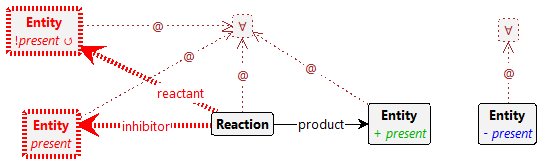
\includegraphics[scale=.40]{react}
\end{center}

To parse this, note that (in the GROOVE rule syntax) the red structure must be absent for the rule to apply; moreover, green labels are added and blue ones deleted upon rule application. The \ilab{present} flag signals whether an \blab{Entity} is considered to be currently present; hence, creating or deleting that flag comes down to creating or deleting the \blab{Entity}. The $\forall$-nodes impose the desired quantification, causing a single application of this rule to model the firing of all enabled \blab{Reaction}s, even if there are thousands of them.

Our model also supports environments that inject \blab{Entity}s in a controlled manner. This is achieved through a second rule, not shown here. A configuration is reachable if it can be constructed by the alternating application of both rules.

\medskip\noindent
Our first results are encouraging: GROOVE seems capable to explore larger Reaction Systems 
%is well beyond what other tools have been able to achieve, 
by halving the analysis time of both reachability and causal analyses.
More precisely, we are able to find a trace towards unwanted patterns (if they exist) among millions of reachable configurations using different heuristics; then, we can also prune the trace to extract a graphical representation of the causal history of that entities, at least as far as reactants are concerned.

\section{Action Points}
\begin{itemize}
\item Develop toy example
\item Think about possible extensions
\end{itemize}


\section{Background}

\subsection{Reaction Systems with Guarded Contexts}

First, we briefly account for the set theoretic definition of Reaction Systems (RSs)~\cite{DBLP:journals/fuin/EhrenfeuchtR07}. Then, we focus on their process algebraic version~\cite{DBLP:journals/tcs/BrodoBF21}, including the recently introduced notion of guarded contexts~\cite{DBLP:conf/cmsb/BowlesBBFGM24}.


\medskip
\noindent
\textbf{RS basics.}
Let $S$ be a finite set of \emph{entities}. 
A \emph{reaction} in $S$ is a triple $a = (R,I,P)$, where $R, I, P\subseteq S$ are finite, non-empty sets and $R \cap I = \emptyset$. 
The sets $R, I, P$ are the sets of \emph{reactants}, \emph{inhibitors}, and  \emph{products}, respectively. 
Without loss of generality, we admit the use of empty sets of reactants and inhibitors.

A Reaction System is a pair ${\cal A} = (S, A)$, where $S$ is the set of entities, and $A$ is a finite set of reactions in $S$.
Given the current state $W\subseteq S$, a reaction $a = (R,I,P)$ is enabled in $W$ if its \emph{enabling predicate}
$
\mathit{en}_a(W)\triangleq\; R \subseteq W\; \wedge\; I \cap W = \emptyset
$
is satisfied, namely, all reactants must be present and all inhibitors absent.
The \emph{result} of the reaction $a$ on the current state $W$ is defined by letting
$
\mathit{res}_a(W) \triangleq\;
P$ if $\mathit{en}_a(W)$, and
$\mathit{res}_a(W) \triangleq\; \emptyset$ otherwise.
The result of all reactions $A$ on the current state $W$, is $\mathit{res}_A(W) \triangleq \cup_{a \in A} \mathit{res}_a(W)$.

The no-permanency principle of RSs dictates that entities disappear if not sustained by some reaction.
Thus, the current state $W=D\cup C$ is determined by the result $D$ of all reactions on the previous state, together with additional entities $C$ provided by the \emph{context}. 
The dynamics of a RS is formalised in terms of {\em interactive processes}.
They are pairs $\pi = (\gamma, \delta)$, where $\gamma\triangleq \{C_i\}_{i\in[0,n]}$ is the {\em context sequence} and $\delta=\{D_i\}_{i\in[0,n]} $ is the {\em result sequence}, s.t.: 
$D_0 = \emptyset$; and 
$D_{i+1} =  \mathit{res}_{A}(D_{i} \cup C_{i})$ for any $i \in [0,n-1]$.
The sequence $\gamma$ represents external interventions, while the sequence $\delta$ is entirely determined by $\gamma$ and $A$.
We call $\tau \triangleq \{W_{i}\}_{i\in[0,n]}$  the \emph{state sequence}, with $W_{i} \triangleq C_{i} \cup D_{i}$ for any $i \in [0, n]$.

\medskip
\noindent
\textbf{Process algebraic RSs.}
Inspired by Plotkin's Structural Operational Semantics (SOS) approach~\cite{DBLP:journals/jlp/Plotkin04a} and process algebras such as CCS~\cite{Milner80}, we derive a Labelled Transition System (LTS) semantics for RSs by means of inductive inference rules. LTS states are terms of an algebra, each transition defines a computation step of the RS and its label records the entities involved in that step.
Following~\cite{DBLP:journals/tcs/BrodoBF21}, we also admit nondeterministic and recursively defined contexts.
%As common, here we replace the recursive construct $\mathsf{rec}~X.~\mathsf{K}$ with context identifiers $X$ drawn from a family of (recursive) definitions $\Delta \triangleq\{X_j=\mathsf{K}_j\}_{j\in J}$, called the environment.
%
\begin{definition}[RS processes]\label{def:LTSforRS}
%Let $S$ be a set of entities. 
\emph{RS processes} are defined by the grammar below:
\[
\mathsf{P}:=[\mathsf{M}]
\qquad
\mathsf{M}:=(R,I,P) \mid D \mid \mathsf{K} \mid \mathsf{M}|\mathsf{M}
\]
\[
\mathsf{K}::=\nil \mid C.\mathsf{K} \mid \mathsf{K}+\mathsf{K} \mid X
\]
where $R$, $I$, $P$, $C$, and $D$ are sets of entities (with $P\neq \emptyset$ and $R\cap I=\emptyset$) and $X$ is a context identifier drawn from a family of (recursive) definitions $\Delta \triangleq\{X_j=\mathsf{K}_j\}_{j\in J}$, called the environment.
\end{definition}

%While in principle reactions, entities and context processes could be seen as components to be handled separately, we prefer to mix them together to provide a compositional account of their interactions.
A RS process  $\mathsf{P}$ embeds a \emph{mixture} process $\mathsf{M}$ obtained as the parallel composition of some reactions $(R,I,P)$, some available entities $D$ (if any), and some \emph{context} $\mathsf{K}$.
We write $\prod_{i\in I} \mathsf{M}_i$ for the parallel composition of all $\mathsf{M}_i$ with $i\in I$. 

A  context process $\mathsf{K}$ is either: 
the nil context $\nil$ that stops the computation;
the prefixed context $C.\mathsf{K}$ that makes the entities $C$ available to the reactions, and then will behave as $\mathsf{K}$ at the next step;
the non-deterministic choice $\mathsf{K}_1+\mathsf{K}_2$ that can behave as either  $\mathsf{K}_1$ or $\mathsf{K}_2$;  
the context identifier $X$ that behaves as $\mathsf{K}$ for $X=\mathsf{K}\in \Delta$.
For example, if $A=\{\mathsf{a}\}.A + \emptyset.A\in \Delta$ and $B=\{\mathsf{b}\}.B + \emptyset.B\in \Delta$, then the context $A | B$ can  offer any combination of $\mathsf{a}$ and $\mathsf{b}$ at each step.


We say that $\mathsf{P}$ and $\mathsf{P}'$ are structurally equivalent, written $\mathsf{P} \equiv \mathsf{P}'$, when they denote the same term up to the laws of Abelian monoids (unit, associativity and commutativity) for  parallel composition $\cdot | \cdot$, with $\emptyset$ as the unit, and the laws of idempotent Abelian monoids for choice $\cdot +\cdot$, with $\nil$ as the unit. We also assume $D_1 | D_2 \equiv D_1\cup D_2$ for any $D_1,D_2\subseteq S$.

\begin{definition}[RSs as RS processes]\label{def:fromRS}
Let ${\cal A} = (S, A)$  be  a RS, and $\pi = (\gamma, \delta)$ an interactive process, with $\gamma = \{C_i\}_{i\in[0,n]}$ and $\delta = \{D_i\}_{i\in[0,n]}$.
%
For any step $i\in[0,n]$, the corresponding RS process $\llbracket {\cal A},\pi \rrbracket_i$ is defined as follows:
$$
\llbracket {\cal A},\pi \rrbracket_i
\triangleq 
[\; \textstyle \prod_{a\in A} a~|~D_i~|~C_i.C_{i+1}.\cdots.C_n.\nil\;]
$$
%
%We write $\llbracket {\cal A},\pi \rrbracket$ as a shorthand for $\llbracket {\cal A},\pi \rrbracket_0$.
\end{definition}


The SOS semantics of  RS processes is defined by the SOS rules in Fig.~\ref{fig:LTSforRS}.

A transition label $\ell$, written $\obs{(D,C)}{R,I,P}$, records:
the sets $D$ of entities currently in the system; 
the set $C$ of entities provided by the context;
the set $R$ of entities whose presence justifies some reactions;
the set $I$ of entities whose absence justifies some reactions;
and the set $P$ of reaction products.
The SOS rules guarantee that if $\mathsf{P}\xrightarrow{\obs{(D,C)}{R,I,P}} \mathsf{P}'$ it holds $\mathit{en}_{(R,I,P)}(D\cup C)$.
%, i.e.:
% {\color{blue}$R\subseteq D\cup C
%    ~\wedge~
%    (D\cup C)\cap I=\emptyset$.}
%Sometimes we abbreviate the pair $(D,C)$ by $W$.
%
\begin{figure*}[t]
	{\footnotesize
		$$  
		\infer[(\textit{\scriptsize{Ent}})]
		{D \xrightarrow{\obs{(D,\emptyset)}{\emptyset,\emptyset,\emptyset}}\emptyset}
		{}
		\qquad
		\infer[(\textit{\scriptsize{Cxt}})]
		{C.\mathsf{K} \xrightarrow{\obs{(\emptyset,C)}{\emptyset,\emptyset,\emptyset}}\mathsf{K}}{}
		$$
        %\smallskip
		$$
		\infer[(\textit{\scriptsize Suml})]
		{\mathsf{K}_1 + \mathsf{K}_2 \xrightarrow{\ell}\mathsf{K}'_1}
		{\mathsf{K}_1 \xrightarrow{\ell}\mathsf{K}'_1}
		\qquad
		\infer[(\textit{\scriptsize Sumr})]
		{\mathsf{K}_1 + \mathsf{K}_2 \xrightarrow{\ell}\mathsf{K}'_2}
		{\mathsf{K}_2 \xrightarrow{\ell}\mathsf{K}'_2}
		\qquad
		\infer[(\textit{\scriptsize Rec})]
		{X \xrightarrow{\ell}\mathsf{K}'}
		{X=\mathsf{K}\in\Delta & \mathsf{K} \xrightarrow{\ell}\mathsf{K}'}
		$$
        %\smallskip
		$$
		\infer[(\textit{\scriptsize Pro})]
		{(R,I,P)  \xrightarrow{\obs{(\emptyset,\emptyset)}{R,I,P}}(R,I,P)\,|\,P}
		{}
		\qquad
		\infer[(\textit{\scriptsize Inh})]
		{(R,I,P)  \xrightarrow{\obs{(\emptyset,\emptyset)}{J,Q,\emptyset}}(R,I,P)}
		{J \subseteq I & Q \subseteq R & J\cup Q\neq \emptyset}
		$$
        %\smallskip
		$$
		\infer[(\textit{\scriptsize Par})]
		{\mathsf{M}_1~|~\mathsf{M}_2\xrightarrow{\ell_1\cup\ell_2} \mathsf{M}'_1~|~\mathsf{M}'_2}
		{\mathsf{M}_1 \xrightarrow{\ell_1} \mathsf{M}'_1 &
		\mathsf{M}_2 \xrightarrow{\ell_2} \mathsf{M}'_2 &
			\ell_1\frown \ell_2 }
		\qquad
		\infer[(\textit{\scriptsize Sys})]
		{[\mathsf{M}]\xrightarrow{\obs{(D,C)}{R,I,P}} [\mathsf{M}']}
		{\mathsf{M}\xrightarrow{\obs{(D,C)}{R,I,P}} \mathsf{M}' &
			R\subseteq D\cup C}
		$$
	}
\caption{SOS semantics of the RS processes.}\label{fig:LTSforRS}
\end{figure*}

%The context $\nil$ has no transition: it stops the execution. 
The rule $(\textit{Ent})$ records the set of current entities $D$.
By rule $(\textit{Cxt})$, a prefixed context process $C.\mathsf{K}$ makes available the entities in $C$ and then reduces to $\mathsf{K}$. 
Rules $(\textit{Suml})$ and $(\textit{Sumr})$ select a move of either the left or the right context, resp., discarding the other process.
By rule $(\textit{Rec})$, a context identifier $X$ behaves according to its defining process $\mathsf{K}$.
The rule $(\textit{Pro})$ assumes the reaction $(R,I,P)$ is enabled: it records its reactants, inhibitors, and products in the label, and leaves the reaction  available at the next step, together with its products $P$.
The rule $(\textit{Inh})$ records in the label the reasons why the reaction $(R,I,P)$ should not be executed: possibly some inhibiting entities $(J \subseteq I)$ are present or some reactants $(Q \subseteq R)$ are missing, with $J \cup Q \neq \emptyset$, as at least one cause is needed.
The rule $(\textit{Par})$ puts two processes in parallel by pooling their labels and joining all labels components. We write $\ell_1\cup\ell_2$ for the component-wise union of labels:
%
{\footnotesize
\[
%\begin{array}{l}
\textstyle
\bigcup_{i=1,2} \obs{(D_i,C_i)}{R_i,I_i,P_i}
%\obs{(D_1,C_1)}{R_1,I_1,P_1}
%\cup
%\obs{(D_2,C_2)}{R_2,I_2,P_2}\\
%\hspace{4.8cm}
\triangleq 
\obs{(D_1\cup D_2,C_1\cup C_2)}{R_1\cup R_2,I_1\cup I_2,P_1\cup P_2}\ .
%\end{array}
\]}


The sanity check $\ell_1\frown\ell_2$ is required to guarantee that labels of reactants and inhibitors are consistent (see definition below):
%
{\footnotesize
\[
%\begin{array}{l}
\obs{(D_1,C_1)}{R_1,I_1,P_1}
\frown
\obs{(D_2,C_2)}{R_2,I_2,P_2}
\triangleq
\textstyle (\bigcup_{i=1,2} D_i\cup C_i \cup R_i) \cap (I_1\cup I_2) = \emptyset .
%\\
%\hspace{5cm}\triangleq 
%(D_1\cup  D_2 \cup C_1 \cup C_2 \cup R_1 \cup R_2) \cap (I_1 \cup I_2) = \emptyset\ .
%\end{array}
\]
}


Finally, the rule $(\textit{Sys})$ checks that all the needed reactants are available in the system ($R \subseteq D\cup C$). Checking the absence of inhibitors  ($(D\cup C)\cap I = \emptyset$) is not necessary, thanks to the sanity check in rule $(\textit{Par})$.
%
%In the following we assume transitions $\mathsf{P}\xrightarrow{\obs{(D,C)}{R,I,P}} \mathsf{P}'$ guarantee that any instance of the rule $(\textit{Inh})$ is applied in a way that maximizes the sets $J$ and $Q$ (see~\cite{DBLP:journals/tcs/BrodoBF21}).
Notably, the SOS semantics matches the set-theoretic dynamics of RSs (as made precise by~\cite[Th.~19]{DBLP:journals/tcs/BrodoBF21}). 


%\begin{theorem}[cf.~\cite{DBLP:journals/tcs/BrodoBF21}]
%\label{the:corr}
%Let ${\cal A}$  be a RS, let $\pi=(\{C_i\}_{i\in[0,n]},\{D_i\}_{i\in[0,n]})$ an interactive process, and let
%$\mathsf{P}_i \triangleq \llbracket {\cal A},\pi \rrbracket_i$ for any $i\in[0,n]$.
%Then, for any $i\in[0,n-1]$:
%%both the following conditions hold:
%\begin{enumerate}
%\item
%if $\mathsf{P}_i \xrightarrow{\obs{(D,C)}{R,I,P}} \mathsf{P}$
% then
%$D=D_i$, $C=C_i$, $P= D_{i+1}$ and
%$\mathsf{P} \equiv \mathsf{P}_{i+1}$;
%\item there exists
%$R,I \subseteq S$ such that 
%$\mathsf{P}_i \xrightarrow{\obs{(D_i,C_i)}{R,I,D_{i+1}}} \mathsf{P}_{i+1}$.
%\end{enumerate}
%\end{theorem}

We enrich the expressiveness of context processes by introducing the possibility to provide some entities \emph{whenever the current state satisfy certain conditions}.
%We start with very simple conditions on current state that need to be satisfied before the context provides a given set  of entities. 
To this aim, we introduce guarded prefixes $(R,I,C).\mathsf{K}$. 
%
\begin{definition}[Guarded contexts]
We update Definition~\ref{def:LTSforRS} by letting:
\[\mathsf{K}::=\nil \mid (R,I,C).\mathsf{K} \mid \mathsf{K}+\mathsf{K} \mid X
\]
\noindent
where $R,I,C\subseteq S$ are possibly empty sets of entities such that $R\cap I=\emptyset$ and $X$ is a context identifier drawn from a predefined environment $\Delta$.
\end{definition}

The similarity with the syntax of reactions is intended: the key difference is that in $(R,I,C).\mathsf{K}$ the presence of reactants $R$ and the absence of inhibitors $I$ is checked w.r.t. the set of current entities $D$.
%instead of $W$ (i.e., $R\subseteq D$ and $D\cap I=\emptyset$) and, 
More importantly, the products $C$ are made available immediately from the context, not at the next step.
We admit $R$ and $I$ to be possibly empty, and abbreviate $(\emptyset,\emptyset,C).\mathsf{K}$ as $C.\mathsf{K}$.
Note that a conditional prefixed process that is not enabled behaves as the $\nil$ process.
%, i.e., there is no rule for $(R,I,C).\mathsf{K}$ that is analogous to rule $(Inh)$ for reactions.
%
%We can now introduce the new syntax for context processes. 




\begin{figure*}[t]
	{\footnotesize
		$$  
		\infer[(\textit{\scriptsize{Ent}})]
		{D \xrightarrow{\obs{\obs{D}{\emptyset,\emptyset,\emptyset}}{\emptyset,\emptyset,\emptyset}}\emptyset}
		{}
		\qquad
		\infer[(\textit{\scriptsize{Cxt}})]
		{(R,I,C).\mathsf{K} \xrightarrow{\obs{\obs{\emptyset}{R,I,C}}{\emptyset,\emptyset,\emptyset}}\mathsf{K}}{}
		$$
    %    {\color{red}%\smallskip
	%	$$
	%	\infer[(\textit{\scriptsize Suml})]
	%	{\mathsf{K}_1 + \mathsf{K}_2 \xrightarrow{\ell}\mathsf{K}'_1}
	%	{\mathsf{K}_1 \xrightarrow{\ell}\mathsf{K}'_1}
	%	\qquad
	%	\infer[(\textit{\scriptsize Sumr})]
	%	{\mathsf{K}_1 + \mathsf{K}_2 \xrightarrow{\ell}\mathsf{K}'_2}
	%	{\mathsf{K}_2 \xrightarrow{\ell}\mathsf{K}'_2}
	%	\qquad
	%	\infer[(\textit{\scriptsize Rec})]
	%	{X \xrightarrow{\ell}\mathsf{K}'}
	%	{X=\mathsf{K}\in\Delta & \mathsf{K} \xrightarrow{\ell}\mathsf{K}'}
	%	$$}
        %\smallskip
		$$
		\infer[(\textit{\scriptsize Pro})]
		{(R,I,P)  \xrightarrow{\obs{\obs{\emptyset}{\emptyset,\emptyset,\emptyset}}{R,I,P}}(R,I,P)|P}
		{}
		\;\;
		\infer[(\textit{\scriptsize Inh})]
		{(R,I,P)  \xrightarrow{\obs{\obs{\emptyset}{\emptyset,\emptyset,\emptyset}}{J,Q,\emptyset}}(R,I,P)}
		{J \subseteq I & Q \subseteq R & J\cup Q\neq \emptyset}
		$$
    %   {\color{red} %\smallskip
	%	$$
	%	\infer[(\textit{\scriptsize Par})]
	%	{\mathsf{M}_1~|~\mathsf{M}_2\xrightarrow{\ell_1\cup\ell_2} \mathsf{M}'_1~|~\mathsf{M}'_2}
	%	{\mathsf{M}_1 \xrightarrow{\ell_1} \mathsf{M}'_1 &
	%	\mathsf{M}_2 \xrightarrow{\ell_2} \mathsf{M}'_2 &
	%		\ell_1\frown \ell_2 }
	%	$$}
        %\smallskip
		$$
		\infer[(\textit{\scriptsize Sys})]
		{[\mathsf{M}]\xrightarrow{\obs{\obs{D}{R',I',C}}{R,I,P}} [\mathsf{M}']}
		{\mathsf{M}\xrightarrow{\obs{\obs{D}{R',I',C}}{R,I,P}} \mathsf{M}' &
		R'\subseteq D &
        R\subseteq D\cup C}
		$$
	}
		\caption{Updated rules to handle guarded contexts (rules $(\textit{Suml})$, $(\textit{Sumr})$, $(\textit{Rec})$ and $(\textit{Par})$ are left unchanged from Fig.~\ref{fig:LTSforRS} and thus omitted).}
		\label{fig:guardforRS2nd}
\end{figure*}

The SOS rules are updated as shown in Fig.~\ref{fig:guardforRS2nd}.
To handle guarded contexts we need a more sophisticated kind of labels: we write $\ell$ for a tuple of the form 
$$\obs{\obs{D}{R',I',C}}{R,I,P}$$
whose novel component $\obs{D}{R',I',C}$ records the available entities $D$ together with those provided by the guarded contexts, assuming all entities in $R'$ are present and those in $I'$ are absent.
%, while the remaining sets $R,I,P$ are as before.
The SOS rules guarantee that whenever $\mathsf{P}\xrightarrow{\obs{\obs{D}{R',I',C}}{R,I,P}} \mathsf{P}'$ it holds that 
$\mathit{en}_{(R',I',C)}(D)$ and
$\mathit{en}_{(R,I,P)}(D\cup C)$.
%, i.e.:
%\begin{equation*}
%R'\subseteq D
%\quad\wedge\quad
%D\cap I'=\emptyset
%\quad\wedge\quad
%R\subseteq D\cup C
%\quad\wedge\quad
%(D\cup C)\cap I=\emptyset
%\end{equation*}
%
Consequently, we overload the notation $\ell_1\frown \ell_2$ and $\ell_1\cup \ell_2$ by letting:
%
{\footnotesize
\[
\begin{array}{l}
\obs{\obs{D_1}{R'_1,I'_1,C_1}}{R_1,I_1,P_1}
\frown
\obs{\obs{D_2}{R'_2,I'_2,C_2}}{R_2,I_2,P_2}
\\
\hspace{1.75cm}\triangleq (\textstyle\bigcup_{i=1,2} D_i\cup  R'_i) \cap (I'_1 \cup I'_2) = \emptyset
\wedge
(\bigcup_{i=1,2} D_i\cup  C_i\cup  R_i) \cap (I_1 \cup I_2) = \emptyset \\[5pt]
\obs{\obs{D_1}{R'_1,I'_1,C_1}}{R_1,I_1,P_1}
\cup
\obs{\obs{D_2}{R'_2,I'_2,C_2}}{R_2,I_2,P_2}
\\
\hspace{1.75cm}\triangleq \obs{\obs{D_1\cup D_2}{R'_1\cup R'_2,I'_1\cup I'_2,C_1\cup C_2}}{R_1\cup R_2,I_1\cup I_2,P_1\cup P_2}
\end{array}
\]}

\begin{example}
The context 
\(
X = (\{\mathsf{a}\},\emptyset,\{\mathsf{b}\}).X + (\{\mathsf{b}\},\emptyset,\{\mathsf{a}\}).X + (\emptyset,\{\mathsf{a},\mathsf{b}\},\emptyset).X
\)
%\noindent
ensures that whenever $\mathsf{a}$ or $\mathsf{b}$ are present in the current state, then both $\mathsf{a}$ and $\mathsf{b}$ are available as reactants.
The last option $(\emptyset,\{\mathsf{a},\mathsf{b}\},\emptyset).X$ handles the case where the first two guards fail: if omitted, when both $\mathsf{a}$ and $\mathsf{b}$ are absent the context $X$ would behave as $\nil$, blocking the computation.
\end{example}


\subsection{Graph Transformation Systems}

\section{Toy Example}

Coffee machine? ATM?

\section{Encoding of RS in GT}
\begin{itemize}
\item Rules for implementing RS semantics
\item Conversion of a trace to a control program
\item Using recipes in the occurrence graph building
\end{itemize}

\section{Comparison}
(\url{https://www.reactionsystems.org/about-reaction-systems})
\begin{itemize}
\item BioReSolve
\item Heresy
\item WebRSim
\item CL-RS (\url{https://github.com/mnzluca/cl-rs})
\item Maude
\end{itemize}

\section{Flexibility of encoding}
\begin{itemize}
\item We can modify our system to other RS variants
\item Do another (small) case study? Durations?
\end{itemize}



\backmatter

\bmhead{Supplementary information}

If your article has accompanying supplementary file/s please state so here. 

\bmhead{Acknowledgements}

\section*{Declarations}

\subsection*{Funding}

Research partially supported 
by \textcolor{red}{Other projects}
by the PRIN PNRR 2022 project \emph{Resource Awareness in Programming} (RAP, P2022HXNSC),
by the University of Pisa PRA project \emph{Formal methods for the healthcare domain based on spatial information} (FM4HD, PRA\_2022\_99),
and by the INdAM GNCS project CUP\_E53C22001930001.

\subsection*{Ethical Approval}
This is not applicable.
 
\subsection*{Competing interests}
The authors have no relevant financial or non-financial interests to disclose.

\subsection*{Availability of data and materials}
Data Availability Statement: No Data associated in the manuscript.

\subsection*{Code availability}

\textcolor{red}{Pointer to git repository?}

\subsection*{Author contribution}

All co-authors contributed equally to this work.

\begin{appendices}

\section{Section title of first appendix}

An appendix contains supplementary information that is not an essential part of the text itself but which may be helpful in providing a more comprehensive understanding of the research problem or it is information that is too cumbersome to be included in the body of the paper.

\end{appendices}


\bibliography{references}



\end{document}
